\begin{wrapfigure}{r}{80mm}
\vspace*{-3mm}
\centerline{
\begin{tabular}{cccc}
    \hspace*{-2mm}  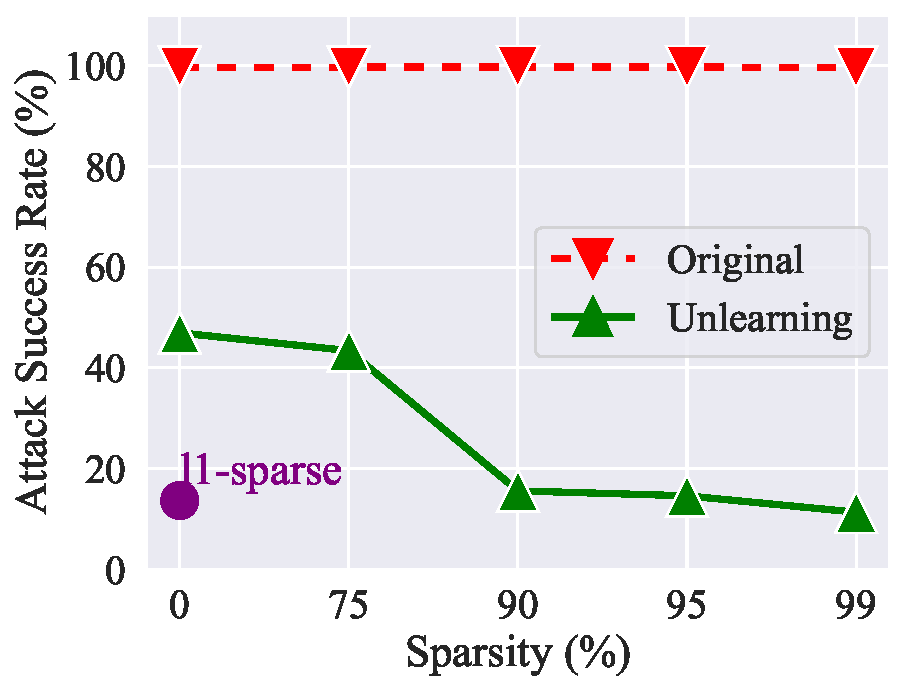
\includegraphics[width=40mm,height=!]{figs/rebuttal/backdoor_ASR.pdf} &
    \hspace*{-5mm} 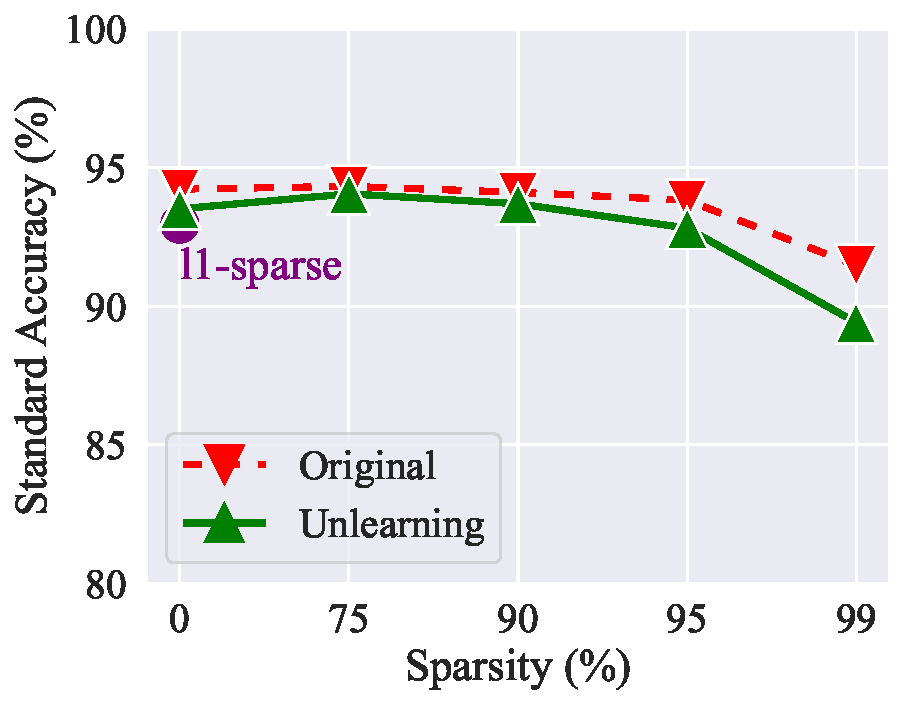
\includegraphics[width=40mm,height=!]{figs/rebuttal/backdoor_SA.pdf} \\

    % \hspace*{-5mm} \includegraphics[width=.25\textwidth,height=!]{figs/placeholder_JC/backdoor_ours_attack_acc.pdf} &
    % \hspace*{-5mm}  \includegraphics[width=.25\textwidth,height=!]{figs/placeholder_JC/backdoor_ours_test_acc.pdf} 
\end{tabular}
}
\vspace*{-2mm}
\caption{
% One figure demonstrates that our methods can decrease attack success rates and maintain good generalization performance.
Performance  of  Trojan model cleanse   via proposed unlearning vs. model sparsity, where `Original' refers to the original Trojan model.
%the effectiveness of the `Unlearn first, then prune' paradigm on the trojan model
%cleanse application. 
\textbf{Left}: ASR vs. model sparsity. \textbf{Right}: SA vs. model sparsity. 
%Each marker represents the mean value over $10$ independent trials. %\JC{Add {\MUSparse}}
%Results  The line and shaded area of each plot represent the mean and variance   over $10$ independent trials. 
%\JC{remove variance}
}
  \label{fig: results_MU_pruning_backdoor}
 \vspace*{-4mm}
%\end{wrapfigure}
%\end{figure}
\end{wrapfigure}